%%%%%%%%%%%%%%%%%%%%%%%%%%%%%%%%%%%%%%%%%%%%%%%%%%%%%%%%%%%%%%%%%%%%%%%%%%%%%%%%%%%%%%%%%%%%%%%%%%%%
% Author: Leon Kuchenbecker <kuchenb@informatik.uni-tuebingen.de>
%%%%%%%%%%%%%%%%%%%%%%%%%%%%%%%%%%%%%%%%%%%%%%%%%%%%%%%%%%%%%%%%%%%%%%%%%%%%%%%%%%%%%%%%%%%%%%%%%%%%
% DOCUMENT CONFIGURATION
%
% ngerman  Set language to "neue deutsche Rechtschreibung". The option is going to be passed to the
%          babel package and makes sure that hyphenation as well as terms such as "Figure", "Table",
%          etc. are properly localized. If you write your document in English, use the "american"
%          option instead.
%
% a4paper  The paper size of the document
%
%    12pt  The default font size (\normalsize)
%%%%%%%%%%%%%%%%%%%%%%%%%%%%%%%%%%%%%%%%%%%%%%%%%%%%%%%%%%%%%%%%%%%%%%%%%%%%%%%%%%%%%%%%%%%%%%%%%%%%

\documentclass[american, a4paper, 12pt]{scrartcl}
%\documentclass[ngerman, 4paper, 12pt]{scrartcl}

%%%%%%%%%%%%%%%%%%%%%%%%%%%%%%%%%%%%%%%%%%%%%%%%%%%%%%%%%%%%%%%%%%%%%%%%%%%%%%%%%%%%%%%%%%%%%%%%%%%%
% PACKAGES
%%%%%%%%%%%%%%%%%%%%%%%%%%%%%%%%%%%%%%%%%%%%%%%%%%%%%%%%%%%%%%%%%%%%%%%%%%%%%%%%%%%%%%%%%%%%%%%%%%%%

% If you want to learn more about how to use a package, your LaTeX distribution already comes with
% an exstensive documentation! Simply enter 'texdoc <packagename>' at the command line and the
% documentation for the requested package will be shown.

% [inputenc] Load this package with the 'utf8' option to write your .tex file with utf8 encoding.
% Recommended for direct handling of umlauts.
\usepackage[utf8]{inputenc}

% Font configuration. Check out http://www.tug.dk/FontCatalogue/ for more fonts and how to configure
% them.
\usepackage{libertine}
\usepackage[T1]{fontenc}

% [babel] This package handles localization as mentioned in the document configuration section.
\usepackage{babel}

% [ams*] The ams packages provide useful commands for typesetting mathematical formulas
\usepackage{amsmath,amsfonts,amssymb,amsthm}

% [geometry] This packages allows you to configure the page margins.
\usepackage[margin=2.5cm]{geometry}

% [lipsum] We use this package to generate the "Lorem Ipsum" text for the example output. You can
% remove this package when you write your own document.
\usepackage{lipsum}
\newcommand\randomtext[1]{\textcolor{gray!80}{\lipsum[#1]}}

% [graphicx] This package provides the \includegraphics command to include graphics from external
% files.
\usepackage{graphicx}

% [caption] Allows to configure how captions are displayed. Here, we set that the label font should
% be bold face formatted and that the caption is formatted as a regular paragraph rather than having
% the label hang out.
\usepackage[labelfont=bf,format=plain]{caption}

% [color] This package provides commands related to color, e.g. \textcolor.
\usepackage{xcolor}

% [natbib] Additional features related to citation. Provides the \citet command and additional,
% configurable bibliography styles
\usepackage[numbers]{natbib}

% [hyperref] Provides PDF links for all references (\ref), citations (\cite) and URLs (\url). The
% reader can click on the referencing word and is forwarded to the desired location. By default,
% hyperref decorates the links by changing their color and adding a visible bounding box. This can
% be disabled using the "hidelinks" option.
\usepackage{hyperref}
\hypersetup{hidelinks}

% [microtype] In a simplified sense, the package improves line breaking in justified text. As a
% recommendation, always include this package.
\usepackage{microtype}
\emergencystretch=1.5em

% [!] ADVANCED [!]
% [tikz] With TikZ you can create complex drawings and figures directly in LaTeX. Have a look at the
% manual!
\usepackage{tikz}
\usetikzlibrary{patterns}

% [!] ADVANCED [!]
% [pgfplots] This package is based on TikZ and allows you to create your plots directly in LaTeX.
\usepackage{pgfplots}
\pgfplotsset{width=7cm,compat=1.15}

% This separate file formats the title and provides the \matriculationnumber and \course commands.
\usepackage{titling}
\newcommand{\matriculationnumber}[1]{\def\matriculationnumbertext{#1}}
\newcommand{\course}[1]{\def\coursetext{#1}}
\pretitle{\hrule height .1em\relax\vskip1em \noindent\Large\sffamily\bfseries}
\posttitle{\par\vskip.7em}
\preauthor{\noindent\large}
\postauthor{\ifx\coursetext\undefined\def\coursetext{unknown}\fi\hfill\emph{\coursetext}\par}
\predate{\ifx\matriculationnumbertext\undefined\def\matriculationnumbertext{\emph{unknown}}\fi\noindent\large Matrikelnummer: \matriculationnumbertext\hfill}
\postdate{\vskip1em\hrule height .1em\relax\vskip1em}



%%%%%%%%%%%%%%%%%%%%%%%%%%%%%%%%%%%%%%%%%%%%%%%%%%%%%%%%%%%%%%%%%%%%%%%%%%%%%%%%%%%%%%%%%%%%%%%%%%%%
% TITLE CONFIGURATION
%%%%%%%%%%%%%%%%%%%%%%%%%%%%%%%%%%%%%%%%%%%%%%%%%%%%%%%%%%%%%%%%%%%%%%%%%%%%%%%%%%%%%%%%%%%%%%%%%%%%

% The title of the document
\title{Lorem ipsum dolor sit amet, consectetuer adipiscing elit}
% The date
\date{WS 2018/19}
% Your name
\author{Max Mustermann}
% Your matriculation number
\matriculationnumber{123456}
% The name of the course
\course{Proseminar Grundlagen der Bioinformatik}

%%%%%%%%%%%%%%%%%%%%%%%%%%%%%%%%%%%%%%%%%%%%%%%%%%%%%%%%%%%%%%%%%%%%%%%%%%%%%%%%%%%%%%%%%%%%%%%%%%%%
% MAIN DOCUMENT
%%%%%%%%%%%%%%%%%%%%%%%%%%%%%%%%%%%%%%%%%%%%%%%%%%%%%%%%%%%%%%%%%%%%%%%%%%%%%%%%%%%%%%%%%%%%%%%%%%%%

\begin{document}

% This command generates the title section based on the configuration above
\maketitle

% The abstract is enclosed in an 'abstract' environment. Place the 200-400 words abstract here.
\begin{abstract}
    \randomtext{1-2}
\end{abstract}

\section{Introduction}
\label{sec:einleitung}


% CITING %%%%%%%%%%%%%%%%%%%%%%%%%%%%%%%%%%%%%%%%%%%%%%%%%%%%%%%%%%%%%%%%%%%%%%%%%%%%%%%%%%%%%%%%%%%

% Use the \cite command to add a reference. You can use multiple reference keys, separated by
% commas, i.e. \cite{A,B}. Do _not_ use \cite{A},\cite{B}. Always replace the space before the \cite
% command with a '~' to prevent line breaks before the reference.

While DNA Sequencing used to be a rather laborious and expensive task, we can now determine the
sequence of billions of base pairs at relatively low cost and within a few
days~\cite{Metzker2010,Schadt2010}. 
\randomtext{3}

% If you want to explicitly mention the reference in your text, use the author name. Do not produce
% text such as 
%    ... In [1] it was shown that ...
% but use the \citet command provided by the natbib package instead:

In his review, \citet{Metzker2010} provides an overview over existing second generation sequencing
technologies and also provides a peak into third generation technologies.
\randomtext{4}

% FIGURES %%%%%%%%%%%%%%%%%%%%%%%%%%%%%%%%%%%%%%%%%%%%%%%%%%%%%%%%%%%%%%%%%%%%%%%%%%%%%%%%%%%%%%%%%%

% To place a figure, include the figure environment directly before the sentence where it is
% referenced for the first time. Do not surround it by empty lines in the source code as those would
% cause a new paragraph to be created. Specify the [tp] argument to preferentially place the figure
% at the top of a page [t] and alternatively on its own page [p]. The \label command must be used
% _after_ the \caption command. Use space efficiently, i.e. place figures next to each other if the
% space permits and label them as sub-figures (a), (b), ...
%
% Use an unbreakable space "~" between "Figure", "Table", etc. and the reference when mentioning it
% in the text.

This definition allows us to compute arbitrary free-end-gaps alignments.
\begin{figure}[tp]
    \centering
    \includegraphics{gfx/figure_alignment_matrix.pdf}
    \caption{
        Special cases of free-end-gaps alignments, \textbf{(a)} an overlap alignment and
        \textbf{(b)} a semi-global alignment. The figure shows an optimal alignment, the edit matrix
        with the entries corresponding to that alignment highlighted, as well as the used cost
        function.
    }
    \label{fig:alignment_matrix}
\end{figure}
Examples for an overlap alignment as well as for a semi-global alignment are shown in
Figure~\ref{fig:alignment_matrix}. Based on this definition we will now further generalize the
concept of a pairwise sequence alignment to the \emph{abracadabra} alignment.

% (English) Note that when referencing a particular figure, table, equation etc by its number, it
% becomes a proper name and is capitalized:
%
% ... as shown in Figure~\ref{fig:name} ...
% ... the figure also shows that there are ...

\randomtext{6-7}

% PARAGRAPHS %%%%%%%%%%%%%%%%%%%%%%%%%%%%%%%%%%%%%%%%%%%%%%%%%%%%%%%%%%%%%%%%%%%%%%%%%%%%%%%%%%%%%%%

% Create a new paragraph by entering an empty line in-between the text.

This is yet another paragraph about very interesting scientific findings. I really have no clue what
to write about here, but I do have to generate some text in order to illustrate how to induce a new
paragraph in \LaTeX. Here it comes.

By placing an empty line in the source code, \LaTeX\ knows that I'd like to start a new paragraph
here. \randomtext{9}

\section{Methods}
\label{sec:methods}

\randomtext{8}

% MATHEMATICAL EQUATIONS %%%%%%%%%%%%%%%%%%%%%%%%%%%%%%%%%%%%%%%%%%%%%%%%%%%%%%%%%%%%%%%%%%%%%%%%%%%

% Use the "align" environment to create an equation that can be referenced, i.e. that is numbered,
% and the "align*" environment to create one that is not numbered. Only use numbered equations if
% you actually reference the equation from the text.
%
% Formulate grammatically correct sentences also if they contain equations! If an equation ends a
% sentence, terminate it with a punctuation mark. If the equation interleaves a sentence, add a
% comma at the end of the equation if necessary.

Therefore, we can now formulate the target function as
\begin{align}
    \mathcal{L}(\mathbf{w},b,\alpha)&=\frac{1}{2}\mathbf{w}^\intercal\mathbf{w}-
    \sum_{i=1}^N\alpha_i(y_i(\mathbf{w}^\intercal\mathbf{x}_i+b)-1), % comma, sentence continues.
    \label{ali:dualOriginal}
\end{align}
where $\alpha_i$ are Lagrange multipliers. Using the partial derivatives for $\mathbf{w}$ and
$b$
\begin{align*}
    \triangledown_\mathbf{w}\mathcal{L}&=\mathbf{w}-\sum_{i=1}^N\alpha_iy_i\mathbf{x}_i=0\\
    \frac{\delta\mathcal{L}}{\delta b}&=-\sum_{i=1}^N\alpha_iy_i=0
\end{align*}
we can simplify Equation~\ref{ali:dualOriginal} as follows:
\begin{align*}
    \mathcal{L}(\alpha)&=\sum_{i=1}^N\alpha_i-\frac{1}{2}\sum_{i=1}^N\sum_{j=1}^Ny_iy_j
    \alpha_i\alpha_j\mathbf{x}_i^\intercal\mathbf{x}_j. % full stop, sentence ends here.
\end{align*}

\randomtext{9-11}

% FIGURE PLACEMENT %%%%%%%%%%%%%%%%%%%%%%%%%%%%%%%%%%%%%%%%%%%%%%%%%%%%%%%%%%%%%%%%%%%%%%%%%%%%%%%%%

% Note that LaTeX may place multiple figures at the top of the page, even though they do not
% directly belong to each other. Do not attempt to manually override the figure placement. The
% separation of figures and text increases readability, as the text flow is not interrupted as
% often.

\begin{figure}[tp]
    \centering
    \includegraphics[width=.4\linewidth]{gfx/public_domain_brain.pdf}
    \caption{
        The human brain. If properly trained, it can solve all kinds of tasks.
    }
    \label{fig:brain}
\end{figure}
Among other organs, humans possess a relatively large brain, as shown in
Figure~\ref{fig:brain}. \randomtext{12}

While training the brain is important, nutrition is another important aspect contributing to brain
function.
\begin{figure}[tp]
    \centering
    \includegraphics[width=.2\linewidth]{gfx/public_domain_broccoli.pdf}\hspace{5mm}
    
\includegraphics[width=.2\linewidth]{gfx/public_domain_corn.pdf}\hspace{5mm}
    \includegraphics[width=.2\linewidth]{gfx/public_domain_tomato.pdf}
    \caption{
        Vegetables (from left to right): broccoli, corn and tomato.
    }
    \label{fig:veggie}
\end{figure}
Vegetables such as broccoli, corn and tomatoes (see Figure~\ref{fig:veggie}) may play an important
role here, or maybe not. \randomtext{13-20}

\section{Evaluation}
\label{sec:Evaluation}

\randomtext{21-24}

% PLOTS %%%%%%%%%%%%%%%%%%%%%%%%%%%%%%%%%%%%%%%%%%%%%%%%%%%%%%%%%%%%%%%%%%%%%%%%%%%%%%%%%%%%%%%%%%%%

% When designing plots, make sure that
%
% - All axis have explanatory labels
% - Legends are present if needed (color, line style, ...)
% - All labels included in the plot (axis, ticks, legends) are _readable_, i.e. the font is large
%   enough and the resolution is sufficiently high!
%
% Below you find an example on how to draw your plot directly in LaTeX, however, this is an advanced
% subject and requires extensive study of the corresponding documentation (pgfplots package). The
% advantage of this approach is that the plot is well integrated into the rest of the document with
% respect to fonts and font sizes.
%
% Another common approach is to generate the plot externally, e.g. using R + ggplot, export it to a
% vector graphic (PDF) (not a bitmap such as PNG!) and then use \includegraphics to include it in
% the document.

\begin{figure}[tp]
    \centering
    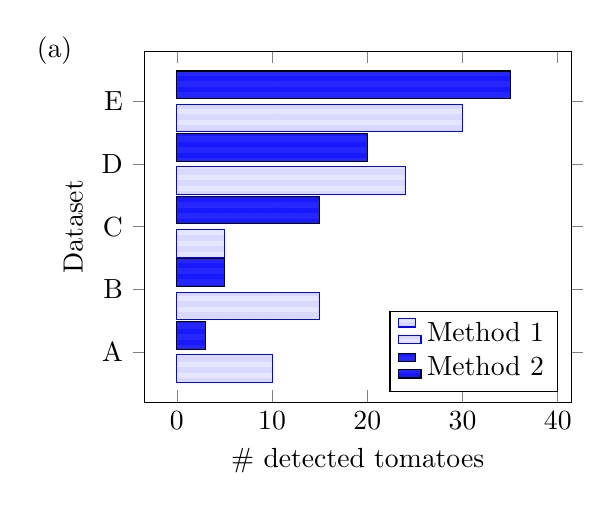
\begin{tikzpicture}
        \begin{axis}[
            xbar,
            enlargelimits=0.20,
            symbolic y coords={A,B,C,D,E},
            ytick=data,
            ylabel=Dataset,
            xlabel={\# detected tomatoes},
            legend pos=south east,
            ]
            \addplot [
                draw=blue,
                pattern=horizontal lines light blue,
                ] coordinates {
                    (10,A) (15,B) (5,C) (24,D) (30,E)
                };
            \addplot [draw=black,
                pattern=horizontal lines dark blue,
                ] coordinates {
                    (3,A) (5,B) (15,C) (20,D) (35,E)
                };
            \legend{Method 1, Method 2}
        \end{axis}
        \node at (current bounding box.north west) {(a)};
    \end{tikzpicture}\hspace{5mm}
    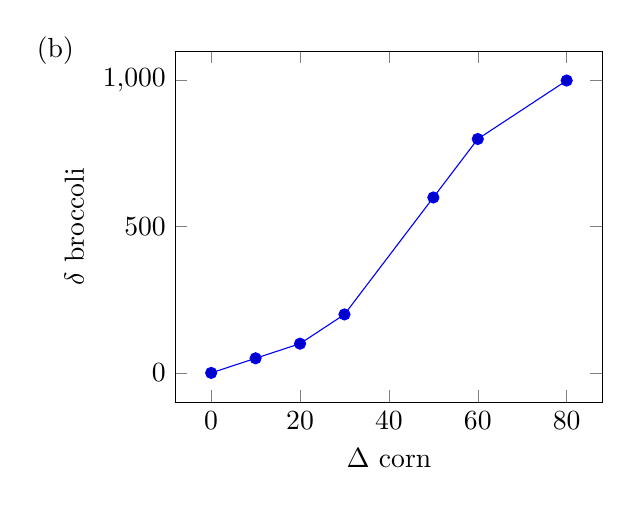
\begin{tikzpicture} 
        \begin{axis}[
            ylabel=$\delta$ broccoli,
            xlabel=$\Delta$ corn,
            ]
            \addplot coordinates {
                    (0,0) (10,50) (20,100) (30,200)
                    (50,600) (60,800) (80,1000)
                };
        \end{axis}
    \node at (current bounding box.north west) {(b)};
    \end{tikzpicture}
    \caption{
        (a) The number of tomatoes detected by either of the two methods across the five main
        datasets. (b) The broccoli coefficient $\delta$ \emph{broccoli} in relation to the corn
        coefficient $\Delta$ \emph{corn}.
    }
    \label{fig:eval}
\end{figure}

A comparison of the two methods is shown in Figure~\ref{fig:eval}(a). \randomtext{25-29}

\section{Discussion}
\label{sec:discussion}

\randomtext{30-41}

% THE BIBLIOGRAPHY %%%%%%%%%%%%%%%%%%%%%%%%%%%%%%%%%%%%%%%%%%%%%%%%%%%%%%%%%%%%%%%%%%%%%%%%%%%%%%%%%

% The bibliography is placed at the end of the document. The \bibliographystyle command chooses the
% style and the \bibliography command points to the input file containing the bib entries.

\bibliographystyle{abbrvnat}
\bibliography{msfx_report}

\end{document}
